\documentclass[12pt]{article}
\usepackage[utf8]{inputenc}
\newcommand\preamble{
    \usepackage[italian]{babel}
    \usepackage{geometry}
    \usepackage{amsmath}
    \usepackage{amssymb}
    \usepackage{graphicx}
    \usepackage{ulem}
    \usepackage[dvipsnames]{xcolor}

    \geometry{margin=2cm}
    \let\olditemize\itemize
    \renewcommand\itemize{\olditemize\setlength\itemsep{0em}}
    \graphicspath{{../Immagini/}}

    \author{Lorenzo Vaccarecci}
}
\preamble

\title{Indici Hash}
\date{12 Aprile 2024}
\begin{document}
\maketitle
\section{Funzione Hash}
\begin{itemize}
    \item \textcolor{red}{distribuzione uniforme} delle chiavi nello spazio negli indirizzi
    \item \textcolor{red}{distrinuzione casuale} delle chiavi (eventuali correlazioni
    tra i valori delle chiavi non devono tradursi in
    correlazioni tra gli indirizzi generati)
\end{itemize}
Una funzione hash è detta \textcolor{red}{perfetta} se non vengono prodotti trabocchi. Può essere sempre definita disponendo di un'area primaria con capacità complessiva pari al numero dei record da memorizzare. Le funzioni hash operano su \textcolor{red}{insiemi di chiavi intere} (se le chiavi sono alfanumeriche si può associare un id prima di applicare la trasformazione).
\subsection{Metodo della divisione}
La chiave numerica viene divisa per $M$ e l'indirizzo è ottenuto considerando il resto:
\begin{equation*}
    H(k)=k \% M
\end{equation*}
\textcolor{Cyan}{Per avere una buona distribuzione delle chiavi è opportuno che $M$ sia un numero primo oppure $\leq 20$.}
\subsection{Costi}
\begin{itemize}
    \item In assenza di overflow, il costo di accesso a indice è \textbf{\textcolor{red}{costante}}.
    \item In presenza di overflow, il costo non è facilmente determinabile. \begin{itemize}
        \item Quanti blocchi di overflow per il blocco acceduto?
        \item Dove sono memorizzati?
    \end{itemize}
\end{itemize}
\section{Creare indirizzi hash}
\begin{itemize}
    \item Specifica della funzione $H$.
    \item Specifica del metodo della gestione dei trabocchi.
    \item Specifica del fattore di caricamento $d$: si intende quanto pieni vogliamo i bucket, se l'istanza della base di dati cambia frequentemente è meglio avere un fattore di caricamento basso ($0\leq d\leq1$). Dipende anche da quanti blocchi il sistema decide di tenere in un bucket.
    \item \textcolor{red}{L'amministratore del database può \textbf{al più} agire la funzione $H$, ma non in tutti i DBMS.}
\end{itemize}
\section{Indici hash clusterizzati e non clusterizzati}
E' \textcolor{red}{clusterizzato} se i record con chiavi simili sono memorizzati nello stesso bucket. In caso contrario è \textcolor{red}{non clusterizzato}.\\
\textit{Finora abbiamo considerato solo gli indici clusterizzati.}
\\\textcolor{Cyan}{Un file dei dati di tipo hash è sempre associato a un indice hash clusterizzato.}
\\\textcolor{red}{In presenza di un indice hash \textbf{clusterizzato} l'organizzazione primaria corrisponde ai record memorizzati nell'area primaria + i record memorizzati negli overflow.}
\section{Esempio}
\begin{center}
    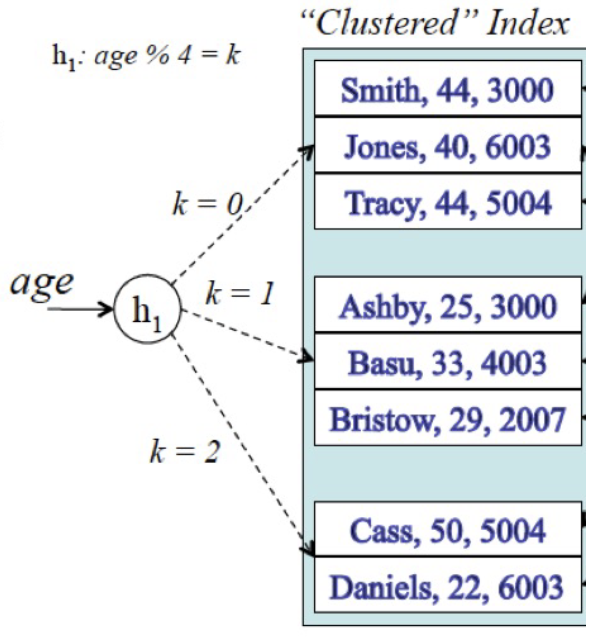
\includegraphics[scale=0.5]{esempioindicihashclusterizzato.png}
    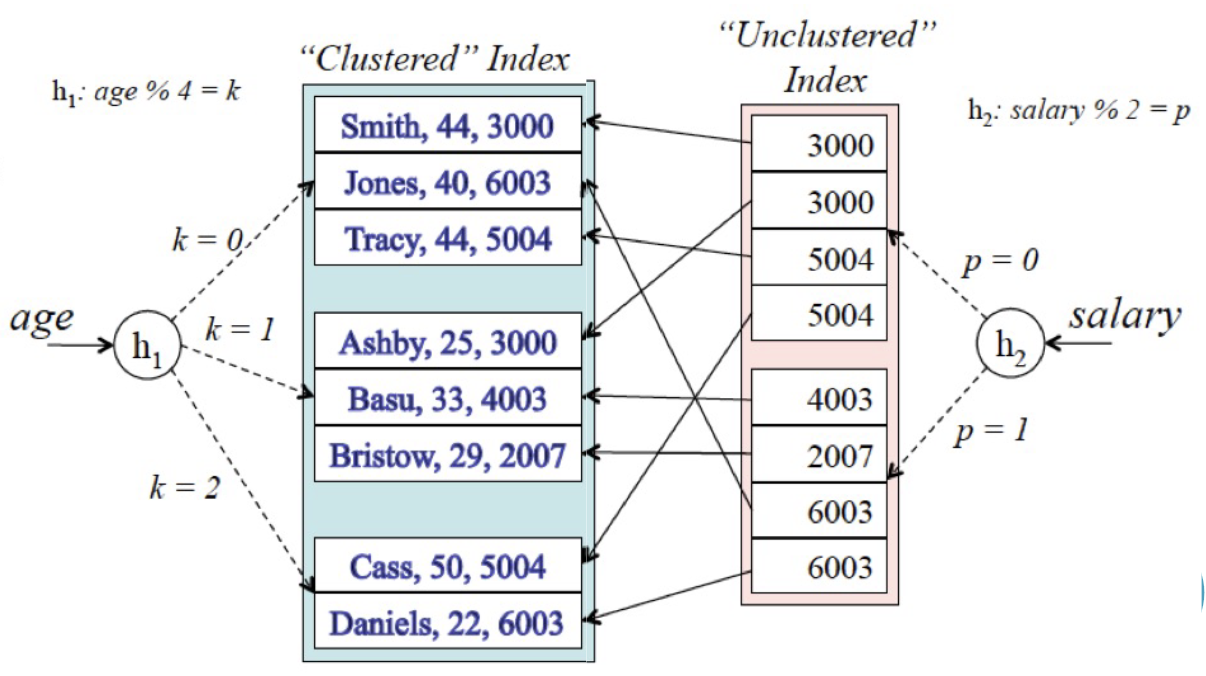
\includegraphics[scale=0.5]{esempioindicihashnonclusterizzato.png}
\end{center}
Gli indici non clusterizzati sono indici multilivello.\\
Per selezioni di uguaglianza sono preferibili gli indici hash, per le selezioni di range sono preferibili gli indici ad albero.
\end{document}